\documentclass{article}
\usepackage[T1]{fontenc}
\usepackage[utf8]{inputenc}
\usepackage{lmodern}
\usepackage{minted}
\usepackage[final]{nips}
\usepackage{outlines}
\usepackage{hyperref}
\usepackage{url}
\usepackage{booktabs}
\usepackage{dsfont}
\usepackage{amsfonts}
\usepackage{nicefrac}
\usepackage{microtype}
\usepackage[dvipdfmx]{graphicx}
\usepackage{float}
\usepackage{lipsum}
\usepackage{caption}
\usepackage{multirow}
\usepackage{graphicx}
\usepackage{amsmath, bm, bbm}
\usepackage{enumitem,amssymb}
\usepackage{pifont}
\newcommand{\cmark}{\ding{51}}
\newcommand{\xmark}{\ding{55}}
\newcommand{\done}{\rlap{$\square$}{\raisebox{2pt}{\large\hspace{1pt}\cmark}}
\hspace{-2pt}}
\newcommand{\wontfix}{\rlap{$\square$}{\large\hspace{1pt}\xmark}}
\captionsetup[table]{position=bottom, skip=2pt}
\hypersetup{colorlinks=true, linkcolor=blue, filecolor=magenta, urlcolor=cyan}
\newcommand{\fixme}[1]{{\color{red} #1}}

\urlstyle{same}
\usemintedstyle{monokai}
\usepackage{booktabs}

\title{Evaluating Adversarial Robustness of Linear Models:\\Sparsity and Kernels}
% Understanding 2020 Poll Results
\author{%
  Shawn Shan, Ziyu Ye \\
  Department of Computer Science\\
  University of Chicago\\
  {shansixiong, ziyuye}@uchicago.edu \\
}
\begin{document}
\maketitle

% %%%%%%%%%%%%%%%%%%%%%%%%%%%%%%%%%%%%%%%%%%%
% \begin{abstract}
% %%%%%%%%%%%%%%%%%%%%%%%%%%%%%%%%%%%%%%%%%%%
% \end{abstract}

%%%%%%%%%%%%%%%%%%%%%%%%%%%%%%%%%%%%%%%%%%%%%
\section{Introduction}
%%%%%%%%%%%%%%%%%%%%%%%%%%%%%%%%%%%%%%%%%%%%%
Robustness is an essential property for a system which indicates if the system can work reliably and stably. In machine learning systems, we are especially concerned about \textbf{adversarial robustness} which considers the robustness of the system when facing adversarial inputs. While there exists rich literature in adversarial attacks in deep neural networks (DNNs)~\cite{hao2020adversarial}, the fundamental principle for adversarial robustness is far from understood.

In this paper, we aim to understand adversarial robustness from the perspective of \textbf{linear models}. We believe our work would help fill the gap of current adversarial robustness study in linear models, and such simplified models should provide relevant insights and heuristics for the more complex scenarios with DNNs.

Specifically, we are interested in how linear models behaves under adversarial attacks with different \textbf{sparsity} and \textbf{kernels}. We choose these two factors as we believe they are fundamental in modern linear models and have close connections to practical DNNs.


%%%%%%%%%%%%%%%%%%%%%%%%%%%%%%%%%%%%%%%%%%%%%
\section{Literature Review}
%%%%%%%%%%%%%%%%%%%%%%%%%%%%%%%%%%%%%%%%%%%%%
\paragraph{Classifier Robustness.} Classifier robustness has been well explored in \fixme{shawn will add this.}

\paragraph{Adversarial robustness of linear models.} ~\cite{biggio2011support} first attempts to attack support vector machines (SVMs) by injecting label noise and propose to improve the robustness by kernel matrix correction. ~\cite{bat2012svm} proposes a poison attack on SVMs by gradient ascent, and ~\cite{liu2017robust} suggests a defense against it by approximating features by a low-rank matrix. Later on, ~\cite{megyeri2019adversarial} shows that linear classifier are less robust when facing higher-dimensional inputs. ~\cite{shi2019understanding} claims that an adversarially robust linear classifier requires higher signal-to-noise ratio, and ~\cite{javanmard2020precise} further confirms this by illustrating the tradeoffs of robustness and accuray for linear models.

\paragraph{The effect of sparsity.} ~\cite{gop2018combating} discusses that learning a sparse representation of input data helps to improve adversarial robustness. ~\cite{guo2018sparse} further illustrates the intrinsic relationship of model sparsity and adversarial robustness.

\paragraph{The effect of kernels.} To the best of our knowledge, we are \textbf{the first} to study the effect of different kernels for linear models under adversarial attacks. Prior work mainly focuses on designing attacks on linear models when kernel is present ~\cite{biggio2011support}, or designing defenses with a certain kernel ~\cite{hao2019defending, taghanaki2019kernelized}.

Based upon the existing literature, our work features by a comprehensive analysis on the family of generalized linear models from the two aspects mentioned above.



%%%%%%%%%%%%%%%%%%%%%%%%%%%%%%%%%%%%%%%%%%%%%
\section{Problem Statement}
%%%%%%%%%%%%%%%%%%%%%%%%%%%%%%%%%%%%%%%%%%%%%
We are interested in how (generalized) linear models behave under different settings of activation, kernel function and sparsity. We consider models from the family of \textbf{Regularized Kernel Regression}.

In evaluating the effect of \textbf{sparsity}, we consider \textit{regularized logistic regression} using $L^{1}$ regularization (\textit{i.e.} lasso regression) or $L^{2}$ regularization (\textit{i.e.} ridge regression); in evaluating the effect of \textbf{kernels}, we consider \textit{kernel logistic regression} using linear, polynomial, Gaussian or sigmoid kernels.



%============================================
\section{Experiment Results}
%============================================
%============================================


\subsection{Datasets and Experiment Setup}
  
\paragraph{Dataset and Classifier. } We use the popular MNIST dataset~\cite{lecun1995mnist}. This task seeks to recognize $10$ handwritten digits in black and white images. The dataset consists of $60,000$ training images and $10,000$ test images. In addition to this, we also use the Iris dataset~\cite{fisher1936uci}, which consists of $150$ images with $3$ classes and $4$ features. We use a multi-class logistic regression (\textit{i.e.} softmax) classifier.

\paragraph{Adversarial Attack Setup. } We implement a simple FGSM attack~\cite{goodfellow2014explaining}. FGSM attack creates an adversarial perturbation for an input $x$ by computing a single step in the direction of the gradient of the model's loss function at $x$ and multiplying the resultant sign vector by a small value $\eta$. The adversarial perturbation $\epsilon$ is generated via:
\begin{equation}
    \epsilon = \eta \cdot \text{sign}(\nabla_x \ell(\model(x), y_t))
\end{equation}

We choose $\eta = 0.05$ in our experiment, the same as previous works~\cite{shan2020gotta,xu2017feature}. As there are more complex and stronger attacks such as CW~\cite{cwattack} attack, however, CW attack has overly complex optimization iterations making standardized evaluation on the model hard. In our experiments, we perform \textit{untargeted} attack. In untargeted attack, the perturbation is successful if the perturbed image gets classified to any class different from the unperturbed one's. 


\paragraph{Evaluation Metrics.} We evaluate the performance of a given model using (1) the adversarial robustness, which is $1$ minus attack success rate of the untargeted FGSM attack and (2) the classification accuracy on normal inputs. 


%============================================
\subsection{The Effect of Sparsity}
%============================================
Denote the loss of logistic regression for a sample dataset $(\bm{X}, \bm{y})$ as $\ell(\bm{w}; \bm{X}, \bm{y})$. In particular, we consider the general multi-classification task using the softmax loss. To control for model sparsity, we introduce $L^{1}$ or $L^{2}$ regularization into the loss function. Thus we have:
\begin{equation}
    \ell(\bm{w}; \bm{X}, \bm{y})=-\frac{1}{m}\left[\sum_{i=1}^{m} \sum_{j=1}^{k} \mathbbm{1}\left\{\bm{y}^{(i)}=j\right\} \log \frac{e^{\theta_{j}^{T} \bm{X}^{(i)}}}{\sum_{l=1}^{k} e^{\theta_{l}^{T} \bm{X}^{(i)}}}\right] + \lambda R(\bm{w})
\end{equation}
The partial derivative can be written as:
\begin{equation}
    \nabla_{\bm{w}_{j}} \ell(\bm{w}; \bm{X}, \bm{y}) = -\frac{1}{m} \sum_{i=1}^{m}\left[\bm{X}^{(i)}\left(\mathbbm{1}\left\{\bm{y}^{(i)}=j\right\}-p\left(\bm{y}^{(i)}=j \mid \bm{X}^{(i)} ; \theta\right)\right)\right]+\lambda \nabla_{\bm{w}_{j}} R(\bm{w})
\end{equation}
If we use  $L^{2}$ regularization:
\begin{equation}
    R(\bm{w}) = \sum_{i=1}^{k} \sum_{j=0}^{n} \bm{w}_{i j}^{2}
\end{equation}
If we use $L^{1}$ regularization:
\begin{equation}
    R(\bm{w}) = \sum_{i=1}^{k} \sum_{j=0}^{n} |\bm{w}_{i j}|
\end{equation}


\begin{figure*}[h!]
  \centering
  \begin{minipage}{0.48\textwidth}
  \centering
  
\includegraphics[width=0.8\textwidth]{placeholder.eps}
  \caption{L1 results for Iris dataset.}
  \label{fig:l1-iris}
  \end{minipage}
  \hfill
  \begin{minipage}{0.48\textwidth}
  \centering
    
\includegraphics[width=0.8\textwidth]{placeholder.eps}
  \caption{L2 results for Iris dataset.}
  \label{fig:l2-iris}
  \end{minipage}
  \hfill
\end{figure*}


\begin{figure*}[h!]
  \centering
  \begin{minipage}{0.48\textwidth}
  \centering
  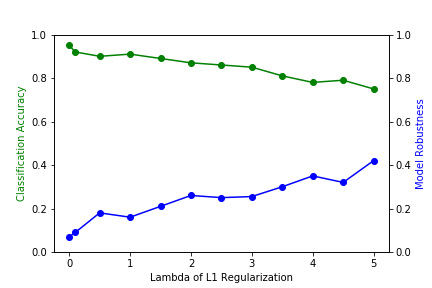
\includegraphics[width=0.8\textwidth]{sparsity_l1.png}
  \caption{Logistic regression classifier's normal classification accuracy and model robustness as lambda increase in $L^{1}$ regularization on MNIST dataset. }
  \label{fig:l1-mnist}
  \end{minipage}
  \hfill
  \begin{minipage}{0.48\textwidth}
  \centering
    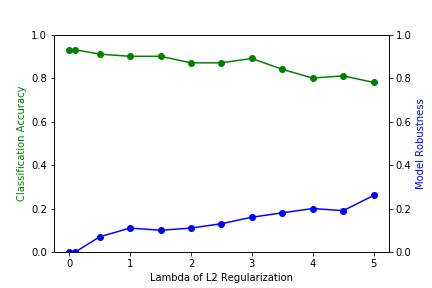
\includegraphics[width=0.8\textwidth]{sparsity.png}
  \caption{Logistic regression classifier's normal classification accuracy and model robustness as lambda increase in $L^{2}$ regularization on MNIST dataset. }
  \label{fig:l2}
  \end{minipage}
  \hfill
\end{figure*}


%============================================
\subsection{The Effect of Kernels}
%============================================
We consider the following kernel functions:
\begin{itemize}
    \item linear kernel: $\kappa (\bm{x}_{i}, \bm{x}_{j})=\bm{x}_{i}^{T}\bm{x}_{j}$
    \item polynomial kernel: $\kappa (\bm{x}_{i}, \bm{x}_{j})=(\bm{x}_{i}^{T}\bm{x}_{j})^{d}$
    \item sigmoid kernel: $\kappa (\bm{x}_{i}, \bm{x}_{j})=\text{tanh}(\beta \bm{x}_{i}^{T}\bm{x}_{j} + \theta)$
\end{itemize}

%============================================
\section{Conclusion}
%============================================
Overall, we have evaluated the adversarial robustness of (generalized) linear models.



%============================================
\newpage
\bibliographystyle{plain}
\bibliography{final}
%============================================

\end{document}
